\documentclass[aspectratio=169]{../latex_main/tntbeamer}  % you can pass all options of the beamer class, e.g., 'handout' or 'aspectratio=43'
\usepackage{dsfont}
\usepackage{bm}
\usepackage[english]{babel}
\usepackage[T1]{fontenc}
%\usepackage[utf8]{inputenc}
\usepackage{graphicx}
\graphicspath{ {./figures/} }
\usepackage{algorithm}
\usepackage[ruled,vlined,algo2e,linesnumbered]{algorithm2e}
\usepackage{hyperref}
\usepackage{booktabs}
\usepackage{mathtools}

\usepackage{amsmath,amssymb}

\DeclareMathOperator*{\argmax}{arg\,max}
\DeclareMathOperator*{\argmin}{arg\,min}

\usepackage{amsbsy}
\newcommand{\vect}[1]{\bm{#1}}
%\newcommand{\vect}[1]{\boldsymbol{#1}}

\usepackage{pgfplots}
\pgfplotsset{compat=1.16}
\usepackage{tikz}
\usetikzlibrary{trees} 
\usetikzlibrary{shapes.geometric}
\usetikzlibrary{positioning,shapes,shadows,arrows,calc,mindmap}
\usetikzlibrary{positioning,fadings,through}
\usetikzlibrary{decorations.pathreplacing}
\usetikzlibrary{intersections}
\pgfdeclarelayer{background}
\pgfdeclarelayer{foreground}
\pgfsetlayers{background,main,foreground}
\tikzstyle{activity}=[rectangle, draw=black, rounded corners, text centered, text width=8em]
\tikzstyle{data}=[rectangle, draw=black, text centered, text width=8em]
\tikzstyle{myarrow}=[->, thick, draw=black]

% Define the layers to draw the diagram
\pgfdeclarelayer{background}
\pgfdeclarelayer{foreground}
\pgfsetlayers{background,main,foreground}

% Requires XeLaTeX or LuaLaTeX
%\usepackage{unicode-math}

\usepackage{fontspec}
%\setsansfont{Arial}
\setsansfont{RotisSansSerifStd}[ 
Path=../latex_main/fonts/,
Extension = .otf,
UprightFont = *-Regular,  % or *-Light
BoldFont = *-ExtraBold,  % or *-Bold
ItalicFont = *-Italic
]
\setmonofont{Cascadia Mono}[
Scale=0.8
]

% scale factor adapted; mathrm font added (Benjamin Spitschan @TNT, 2021-06-01)
%\setmathfont[Scale=1.05]{Libertinus Math}
%\setmathrm[Scale=1.05]{Libertinus Math}

% other available math fonts are (not exhaustive)
% Latin Modern Math
% XITS Math
% Libertinus Math
% Asana Math
% Fira Math
% TeX Gyre Pagella Math
% TeX Gyre Bonum Math
% TeX Gyre Schola Math
% TeX Gyre Termes Math

% Literature References
\newcommand{\lit}[2]{\href{#2}{\footnotesize\color{black!60}[#1]}}

%%% Beamer Customization
%----------------------------------------------------------------------
% (Don't) Show sections in frame header. Options: 'sections', 'sections light', empty
\setbeamertemplate{headline}{empty}

% Add header logo for normal frames
\setheaderimage{
	% 
\includegraphics[height=\logoheight]{figures/TNT_darkv4.pdf}
	
\includegraphics[height=\logoheight]{../latex_main/figures/luh_logo_rgb_0_80_155.pdf}
	% 
\includegraphics[height=\logoheight]{figures/logo_tntluh.pdf}
}

% Header logo for title page
\settitleheaderimage{
	% 
\includegraphics[height=\logoheight]{figures/TNT_darkv4.pdf}
	
\includegraphics[height=\logoheight]{../latex_main/figures/luh_logo_rgb_0_80_155.pdf}
	% 
\includegraphics[height=\logoheight]{figures/logo_tntluh.pdf}
}

% Title page: tntdefault 
\setbeamertemplate{title page}[tntdefault]  % or luhstyle
% Add optional title image here
%\addtitlepageimagedefault{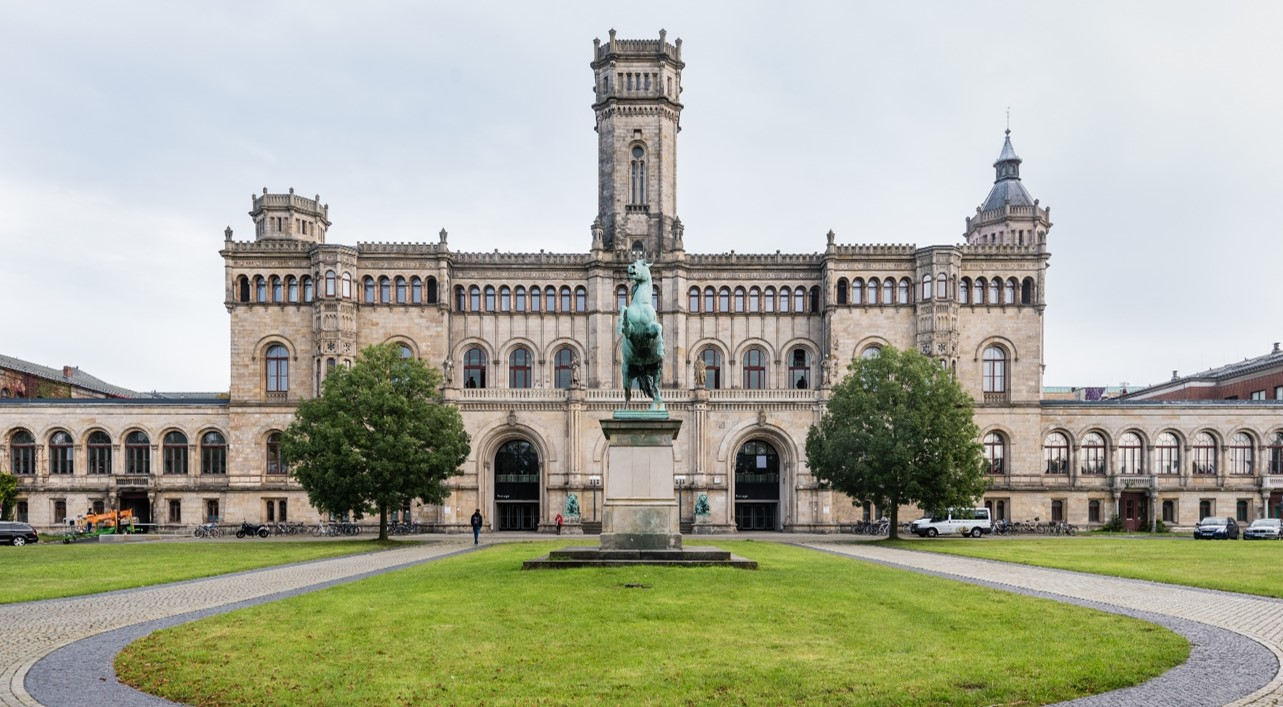
\includegraphics[width=0.65\textwidth]{figures/luh_default_presentation_title_image.jpg}}

% Title page: luhstyle
% \setbeamertemplate{title page}[luhstyle]
% % Add optional title image here
% \addtitlepageimage{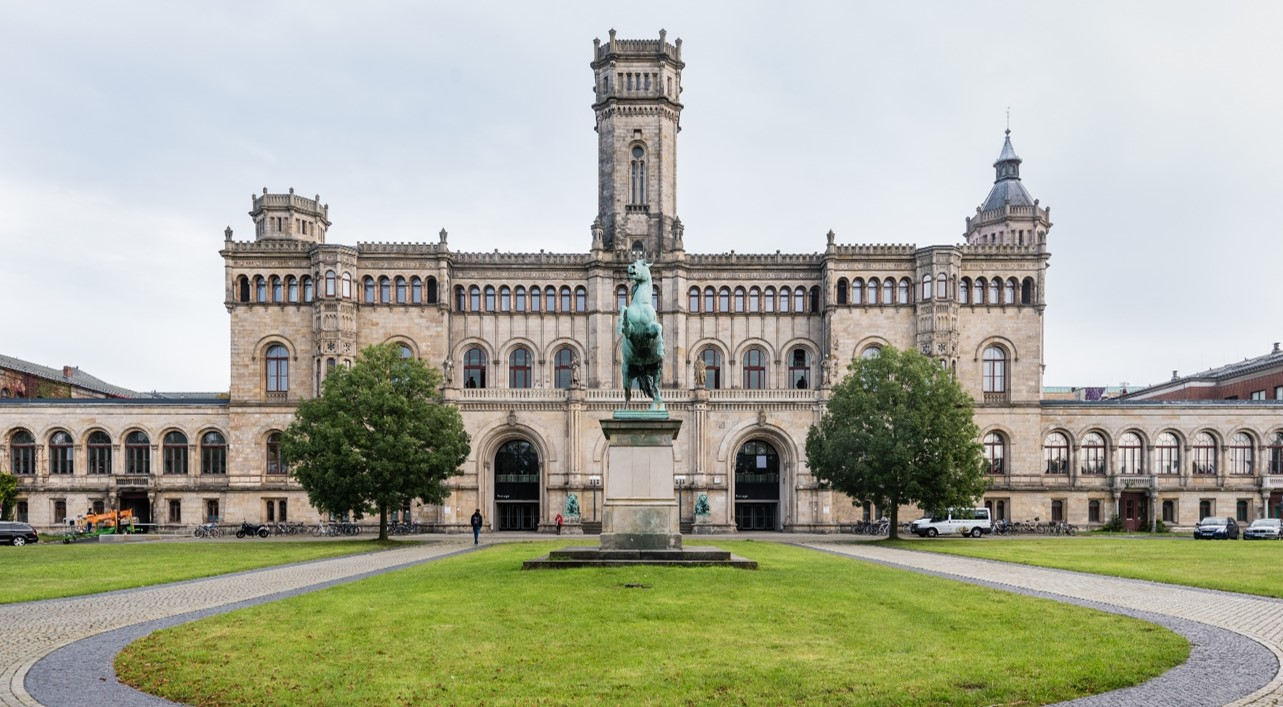
\includegraphics[width=0.75\textwidth]{figures/luh_default_presentation_title_image.jpg}}

\author[Abedjan \& Lindauer]{Ziawasch Abedjan \& Marius Lindauer\\[1em]
	
\includegraphics[height=\logoheight]{../latex_main/figures/luh_logo_rgb_0_80_155.pdf}\qquad
	
\includegraphics[height=\logoheight]{../latex_main/figures/DBIS_Kurzlogo.png}\qquad

\includegraphics[height=\logoheight]{../latex_main/figures/TNT_darkv4}\qquad

\includegraphics[height=\logoheight]{../latex_main/figures/L3S.jpg}	}
\date{Summer Term 2022; \hspace{0.5em} {
\includegraphics[height=1.5em]{../latex_main/figures/Cc-by-nc-sa_icon.svg.png}}; based on \href{https://ds100.org/fa21/}{[DS100]}
}


%%% Custom Packages
%----------------------------------------------------------------------
% Create dummy content
\usepackage{blindtext}

% Adds a frame with the current page layout. Just call \layout inside of a frame.
\usepackage{layout}


%%% Macros
%\renewcommand{\vec}[1]{\mathbf{#1}}
% \usepackage{bm}
%\let\vecb\bm

\title[Introduction]{DS: Principal Component Analysis}
\subtitle{Motivating PCA}

\graphicspath{ {./figure/} }
%\institute{}


\begin{document}
	
	\maketitle
	\begin{frame}{Dimensionality}
	    \begin{columns}
	        \begin{column}{.5\textwidth}
	               Consider the data shown. How many dimensions does this data have?
	               \begin{itemize}
	                   \item 3, because 2 weight columns are redundant
	                   \item In linear algebra terms, we’d observe that this matrix has rank 3
	                   \item More generally: Can think of a dataset’s dimensionality as the rank of the matrix representing the data 
	               \end{itemize}
	        \end{column}
	        
	        
	        \begin{column}{.5\textwidth}
	                \begin{figure}
	                    \centering
	                    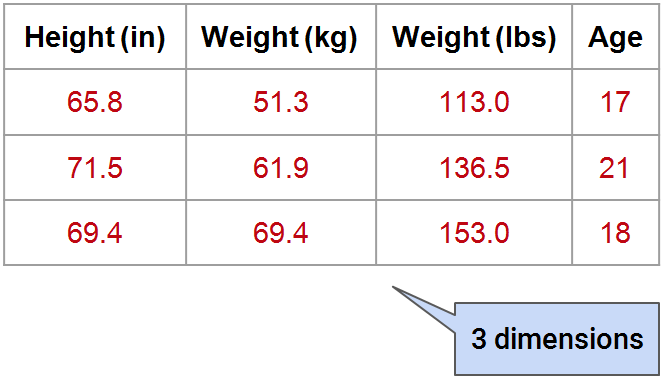
\includegraphics[scale=.4]{Bild4}
	                \end{figure}
	        \end{column}
	    \end{columns}
	\end{frame}
	
	
	\begin{frame}{Dimensionality}
	    \begin{columns}
	        \begin{column}{.5\textwidth}
	               In the previous example, we had one column that was exactly linearly dependent on another.\\
	               \bigskip
	               More generally, we want to summarize data with fewer dimensions, even if no obvious redundancies exist.
	        \end{column}
	        
	        
	        \begin{column}{.5\textwidth}
	                \begin{figure}
	                    \centering
	                    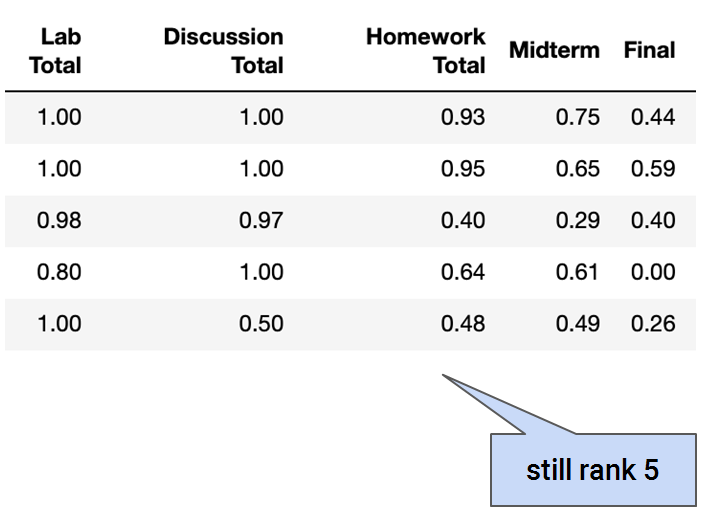
\includegraphics[scale=.4]{Bild5}
	                \end{figure}
	        \end{column}
	    \end{columns}
	\end{frame}
	
	
	\begin{frame}{Summarizing Our Data}
	    We want to summarize each student with a single “score.”
	    \begin{itemize}
	        \item We usually have a predetermined rubric (e.g. 40\% HW, 24\% Final, 10\% Discussion, etc.)
	        \item Notice the rubric is a linear combination of the features for each student.
	    \end{itemize}
	    BUT, what if we wanted a different score, one number that captures the student’s relative performance as comprehensively as possible?\\
	    \bigskip
	    We want to find a linear combination that maximizes the variance of this score.\\
	    \hfill 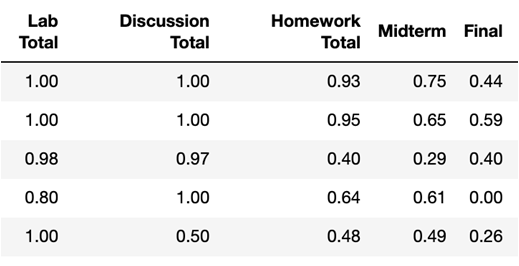
\includegraphics[scale=.6]{Bild6}
	\end{frame}
	
	
	\begin{frame}{Summarizing Our Data}
	    \begin{columns}
	        \begin{column}{.5\textwidth}
	               Let’s say we wanted to assign the “score” based only on the midterm and final exam.\\
	               \bigskip
	               Here, you can see how different linear combinations of the midterm and final affect the variance of our score.\\
	               \bigskip
	               The variance seems to be maximized when our arrow points up and to the right (or down and to the left).\\
	               \bigskip
	               We still don’t know precisely which vector we should use.
	        \end{column}
	        
	        
	        \begin{column}{.5\textwidth}
	        
	                    \centering
	                    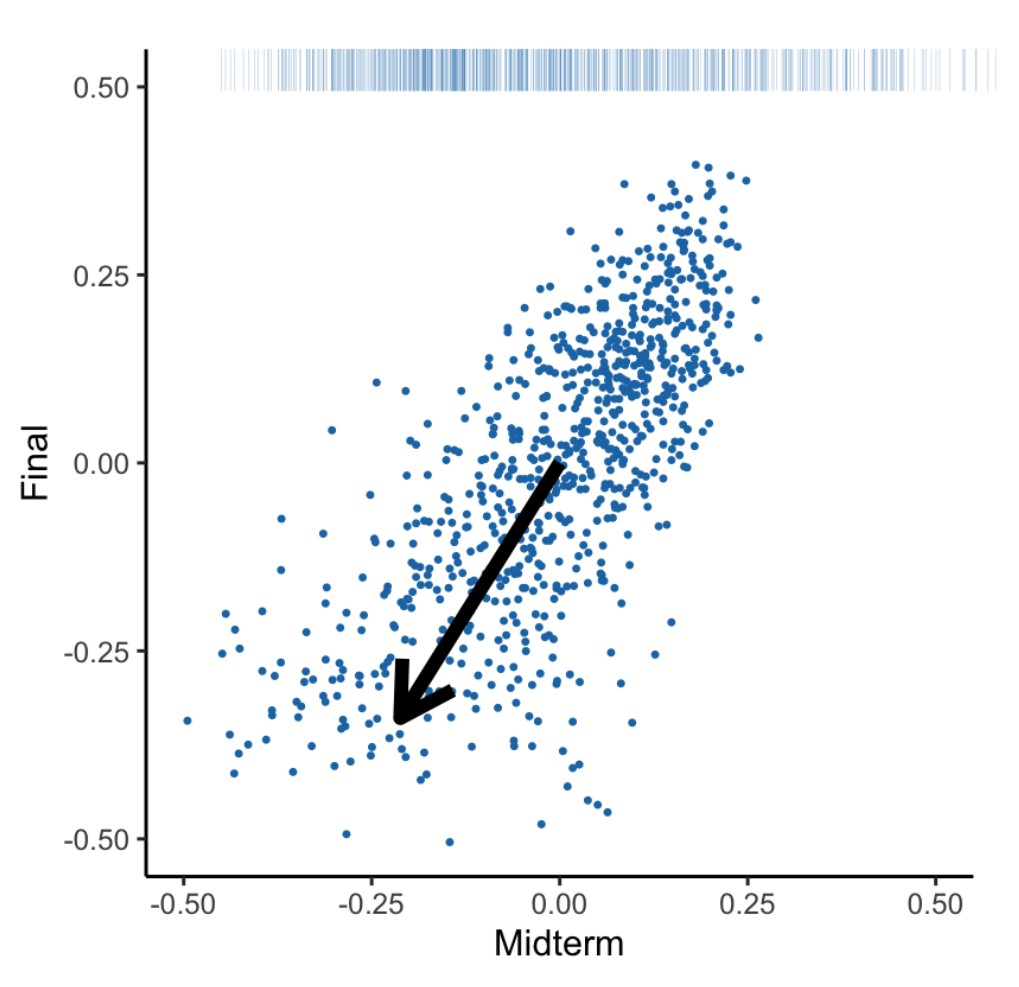
\includegraphics[scale=.1]{vect1}
	                    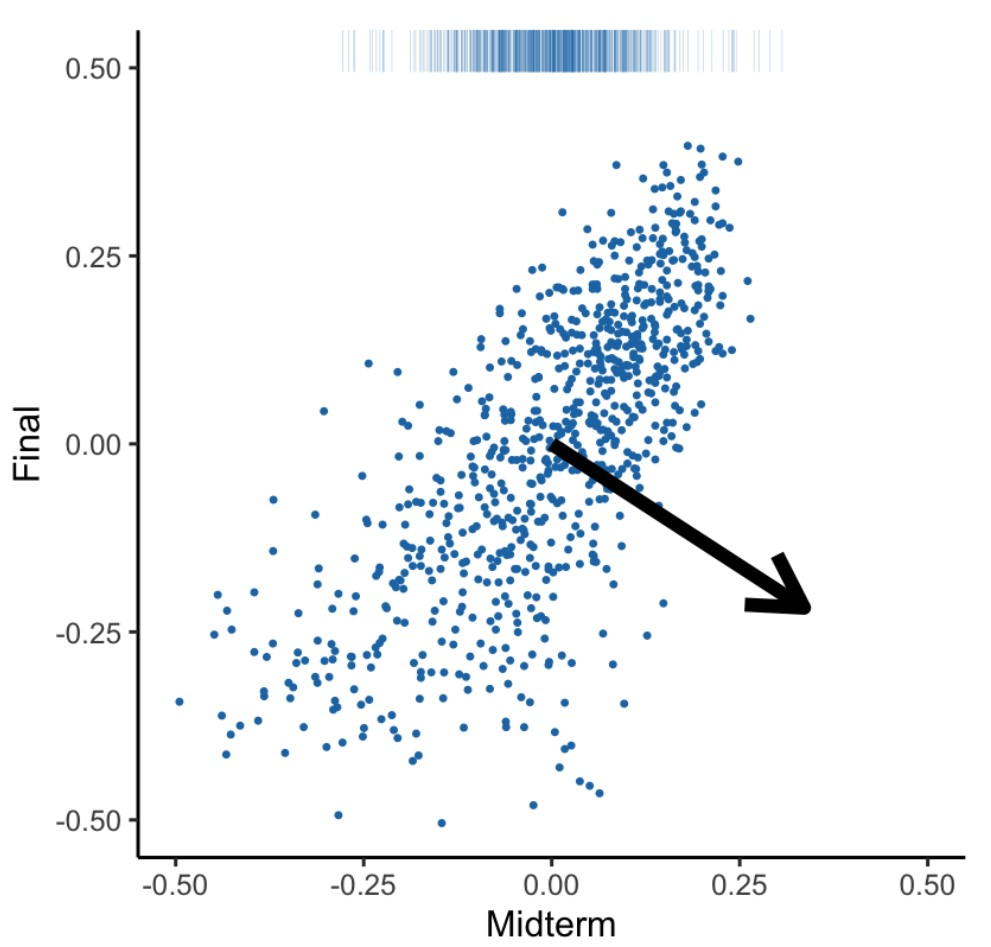
\includegraphics[scale=.1]{vect2}
	                    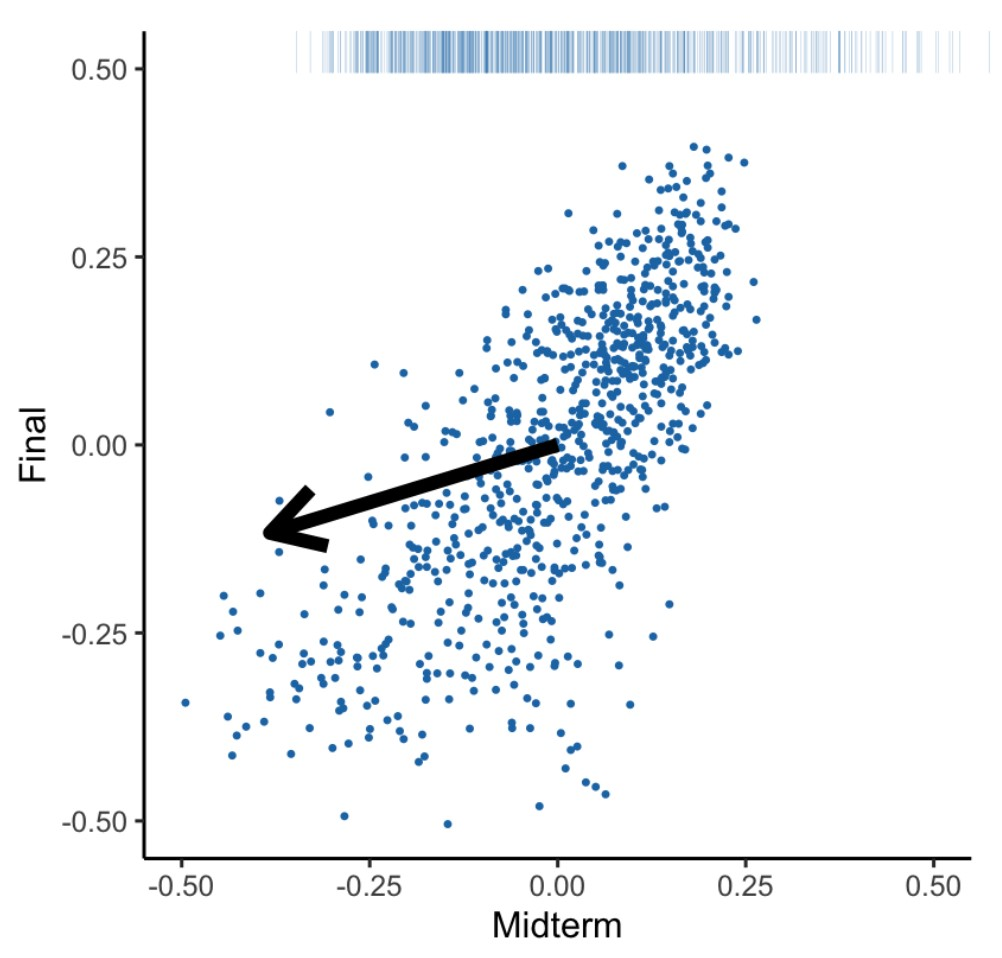
\includegraphics[scale=.1]{vect3}
	                    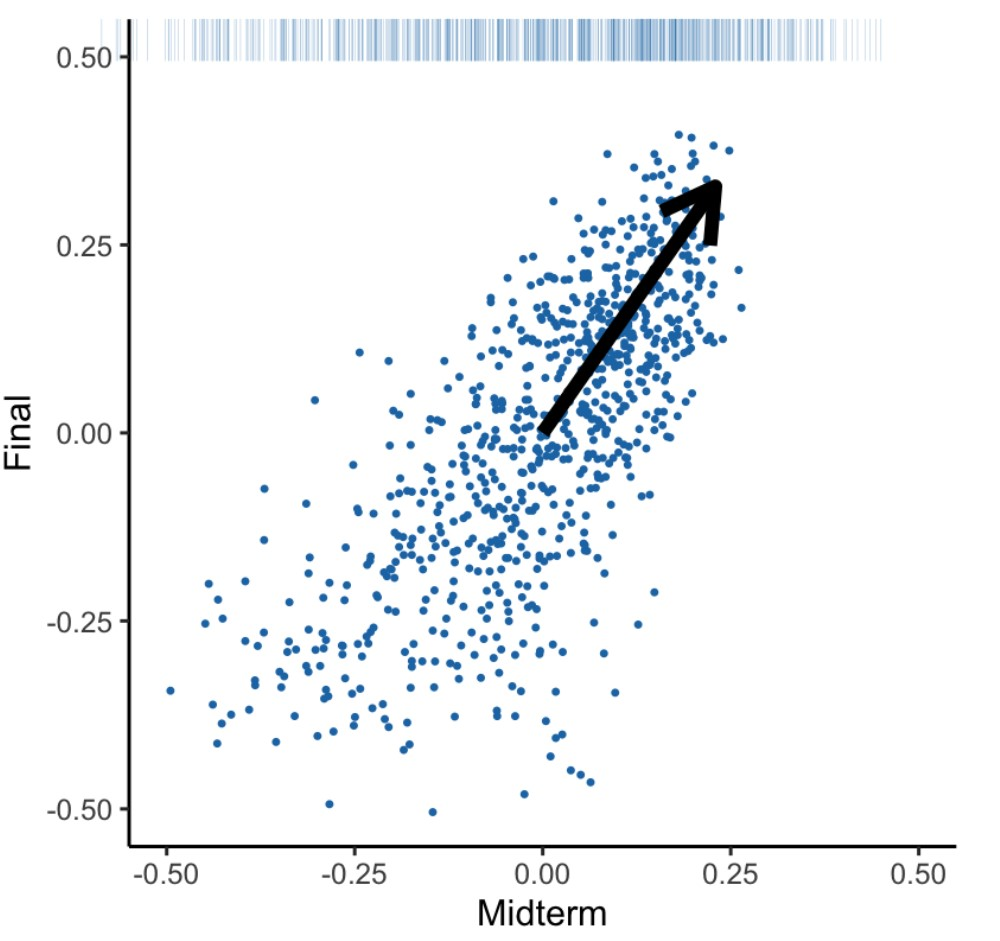
\includegraphics[scale=.1]{vect4}
	                    
	        \end{column}
	    \end{columns}
	\end{frame}
	
	
	\begin{frame}{Connection to SVD}
	    \begin{columns}
	        \begin{column}{.5\textwidth}
	               \begin{equation*}
	                   X = U\Sigma V^T
	               \end{equation*}
	               The long black arrow is the first row in $V^T$.
                  \begin{equation*}
                      v_1^T = [\begin{array}{cc}
                          0.573 & 0.820
                      \end{array}]
                  \end{equation*}
                  The first row of $V^T$ is the direction that captures the most variance in our data.
                  (Note: There exists a proof, but we will not cover it here.)

	        \end{column}
	        
	        
	        \begin{column}{.5\textwidth}
	                \begin{figure}
	                    \centering
	                    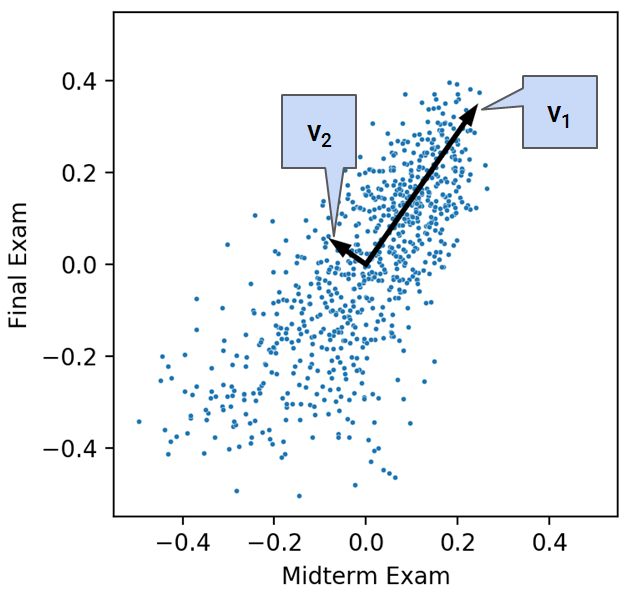
\includegraphics[scale=.35]{Bild8}
	                \end{figure}
	        \end{column}
	    \end{columns}
	\end{frame}
	
	
	
	\begin{frame}{Calculating Our Scores}
	    \begin{columns}
	        \begin{column}{.5\textwidth}
	               Now, we know that $v_1$ tells us the linear combination that maximizes variance. But how do use $v_1$ to compute the “score”?\\
	               \bigskip
	               Treat $v_1$ as an axis and find where each blue data point lies along it.
	               \begin{itemize}
	                   \item We project each data point onto v1, using the formula on the right, converting blue points to purple points.
	                   \item $x_1$’s “score” is	$x_1\cdot v_1$		, which is also the coordinate of $x_1$ along the $v_1$ axis.
	               \end{itemize}


	        \end{column}
	        
	        
	        \begin{column}{.5\textwidth}
	                \begin{figure}
	                    \centering
	                    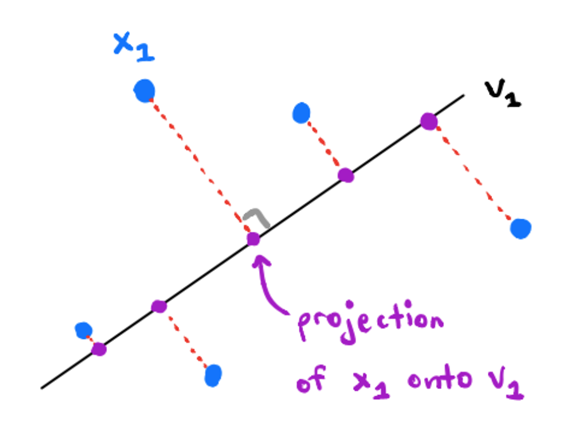
\includegraphics[scale=.4]{Bild9}
	                \end{figure}
	                \begin{align*}
	                    proj_{v_1} x_1 &= \left(\frac{x_1\cdot v_1}{\| v_1 \| ^2}\right)v_1
	                \end{align*}
	                $x_1$: $x_1$ score\\
	                $\| v_1 \|$: equal to 1
	        \end{column}
	    \end{columns}
	\end{frame}
	
	
	\begin{frame}{Calculating Our Scores}
	    Let’s consider the following student : $x^T_{Dr. Doofenshmirtz} = [\begin{array}{cc}
	       0.2  & -0.05
	    \end{array}]$\\
	    This means the student scored 20 percentage points above average on the midterm, and 5 percentage points below average on the final.\\
        Recall, $v_1^T = [\begin{array}{cc}
	       0.573  & 0.820
	    \end{array}] $\\
	    \bigskip
	    To calculate the student’s score, we perform the following calculation:\\
	    $x_{Dr. Doofenshmirtz} \cdot v_1 = \left[\begin{array}{c}
	         0.2  \\
	         -0.05
	    \end{array}\right] \cdot \left[\begin{array}{c}
	         0.573  \\
	         0.820
	    \end{array}\right] = 0.573\times 0.2 + 0.820\times -0.05 = 0.074 $\\
	    \bigskip
	    (The mean score across all students will be 0, if we wanted to convert this into an actual grade, we could shift every score up by some constant.)
	\end{frame}
	
	
	\begin{frame}{Matrix Algebra}
	    To calculate the score for every student, we can use matrix operations.
	    \begin{equation*}
	        Xv_1 = \left[\begin{array}{ccc}
	            \dots & x_1 & \dots \\
	            \dots & x_2 & \dots \\
	                  & \vdots & \\
	            \dots & x_n  & \dots
	        \end{array}\right] \cdot \left[\begin{array}{c}
	             \vdots\\
	             v_1\\
	             \vdots
	        \end{array}\right] = \left[\begin{array}{c}
	             x_1 \cdot v_1\\
	             x_2 \cdot v_1\\
	             \vdots\\
	             x_n \cdot v_1
	        \end{array}\right]
	    \end{equation*}
	    X is centered\\
	    \bigskip
	    The $i^{th}$ element in the vector on the right is the score for the $i^{th}$ student.\\
        (We’ll give this vector a name later.)
	\end{frame}
\end{document}